% =====================================================================
% DNAK v2: Delaunay-Neighbor Accelerated K-means
% Target: Pattern Recognition Letters / Information Sciences (Elsevier)
% Author: Barun Kr Paul (NITTTR Kolkata)
% STATUS: draft with REAL measured results (3 seeds, exactness verified
%         on every run). [TODO] items remain before submission.
% =====================================================================
\documentclass[review,12pt]{elsarticle}
\usepackage{amsmath,amssymb,amsthm}
\usepackage{graphicx}
\usepackage{booktabs}
\usepackage{algorithm}
\usepackage{algpseudocode}
\usepackage{hyperref}
\newtheorem{theorem}{Theorem}
\newtheorem{lemma}{Lemma}
\newdefinition{definition}{Definition}
\journal{Pattern Recognition Letters}

\begin{document}
\begin{frontmatter}
\title{DNAK: Exact Acceleration of Lloyd's $k$-Means in Linear Memory
via Delaunay-Neighbor Pruning}

\author[1]{Barun Kr Paul\corref{cor1}}
\ead{[TODO: email]}
\cortext[cor1]{Corresponding author}
\affiliation[1]{organization={National Institute of Technical Teachers'
Training and Research (NITTTR)}, city={Kolkata}, country={India}}
% [TODO: add supervisor / co-authors]

\begin{abstract}
Exact accelerations of Lloyd's $k$-means algorithm prune redundant
point-to-centroid distance computations without changing the output;
existing exact methods derive their candidate sets from numerical
distance bounds. We propose DNAK (Delaunay-Neighbor Accelerated
$K$-means), which derives them structurally: a greedy walk on the
Delaunay graph of the centroids provably reaches the exact nearest
centroid while visiting only a constant number of candidates on
average, and an order-2 Voronoi property yields \emph{exact}
second-nearest lower bounds in $O(n)$ memory. We prove DNAK reproduces
Lloyd's assignments at every iteration. A compiled six-method
comparison (Lloyd's, Hamerly's, Elkan's, Yinyang, Exponion, DNAK;
exactness verified on every run) shows DNAK consistently outperforming
Hamerly's, Elkan's and Yinyang's algorithms in wall-clock terms, and a
$k$-sweep locates a crossover against Exponion, the strongest prior
low-dimensional method: in the plane DNAK becomes the fastest method
for $k\gtrsim 100$, and because its per-point candidate set is the
$O(1)$ Delaunay neighbourhood while annulus-based candidate sets grow
with $k$, its advantage widens with $k$, reaching $1.8\times$ over
Exponion at $k{=}512$ ($33.3\times$ versus $18.2\times$ speedup over
Lloyd's algorithm). At $d{=}3$ Exponion remains faster at the tested
$k\le 256$, with the gap narrowing as $k$ grows; the difference is
attributable to per-iteration Delaunay reconstruction, whose lazy
variant we analyse via a stale-graph certificate lemma, finding it
profitable only where graph construction dominates ($d{=}4$). The
contribution is a provably minimal structural pruning mechanism with
exact bounds that defines the state of the art for large-$k$ planar
clustering.
\end{abstract}

\begin{keyword}
$k$-means \sep Lloyd's algorithm \sep Delaunay triangulation \sep
Voronoi diagram \sep computational geometry \sep exact acceleration
\end{keyword}
\end{frontmatter}

% =====================================================================
\section{Introduction}
\label{sec:intro}

The $k$-means problem seeks centroids $C=\{c_1,\dots,c_k\}\subset
\mathbb{R}^d$ minimising $\mathrm{SSE}(C)=\sum_i \min_j \lVert
x_i-c_j\rVert^2$ over data $X=\{x_1,\dots,x_n\}$. Lloyd's algorithm \cite{lloyd} alternates assignment (each point to its nearest centroid) and update
(each centroid to its cluster mean). The assignment step costs
$\Theta(nkd)$ per iteration and dominates runtime, yet in late
iterations centroids barely move and almost no point changes cluster,
so most of this work is provably redundant.

Exact accelerators eliminate this redundancy without changing the
output. The two canonical bound-based methods bracket a trade-off.
Elkan's algorithm maintains one upper bound and $k$ lower bounds per
point: pruning is aggressive, but memory is $O(nk)$ and --- crucially
--- \emph{every} bound must be corrected by centroid drift every
iteration, an $O(nk)$ cost paid regardless of how many distances are
actually avoided. Hamerly's algorithm keeps a single lower bound per
point, reducing state and maintenance to $O(n)$, but a bound failure
triggers a full $k$-way rescan.

This paper asks whether computational geometry can break that
trade-off: can an algorithm with Hamerly's $O(n)$ footprint avoid
Hamerly's $O(k)$ fallback? Our answer is DNAK. Its key structural
facts are classical: the Voronoi diagram of the centroids determines
the assignment step; a point's second-nearest centroid is always a
Delaunay neighbour of its nearest (an order-2 Voronoi property); and a
greedy walk on the Delaunay graph from any start provably terminates
at the true nearest centroid. DNAK combines these with drift-tightened
bounds so that a skipped point costs nothing, a re-examined point
costs an $O(1)$-size neighbourhood walk rather than a $k$-way scan,
and every recomputed bound is \emph{exact} rather than merely valid.

\paragraph{Contributions}
(1)~DNAK, an exact accelerator of Lloyd's algorithm with $O(n)$ state
whose fallback cost is the Delaunay degree, not $k$.
(2)~Correctness proofs: greedy-walk exactness, exact second-nearest
bounds via the order-2 Voronoi property, and iteration-by-iteration
equivalence to Lloyd's algorithm (under general position, with a
deterministic tie-breaking rule handling degenerate data).
(3)~A controlled study on synthetic and real data, with a two-metric
evaluation (distance computations and total operations) showing that
DNAK dominates Hamerly's algorithm on both metrics, and dominates
Elkan's algorithm on total work and memory while conceding raw
distance counts --- an honest characterisation of where each method
wins.

% =====================================================================
\section{Related Work}
\label{sec:related}

\paragraph{Bound-based exact accelerators}
Several exact acceleration methods reduce the number of distance
computations in $k$-means. Elkan's algorithm \cite{elkan} uses the
triangle inequality and maintains $O(nk)$ bounds; Hamerly's algorithm
\cite{hamerly} reduces this storage to $O(n)$ with a single lower
bound per point, and the annulus method of Drake and Hamerly
\cite{drake} restricts the rescan to a norm-ordered annulus. Yinyang
$k$-means \cite{yinyang} groups centroids and uses group-level bounds,
while Exponion \cite{newling} limits the search to a ball around the
previously assigned centroid; the Shallot algorithm \cite{borgelt}
further tightens this construction. Bottesch et al.\ \cite{bottesch}
obtain cheaper bounds from norms and block vectors, and the bounding
framework has recently been carried to spherical $k$-means
\cite{schubert} and to exact acceleration of the seeding step itself
\cite{raff,corominas}. All of these derive candidate sets from
numerical bound values. DNAK instead derives them structurally from
the Delaunay graph of the current centroids, so the fallback cost is
governed by the Delaunay degree rather than by $k$. The maintenance
asymmetry matters: per iteration Elkan performs $\Theta(nk)$ bound
updates against $\Theta(n)$ for Hamerly and DNAK, and previous studies
\cite{hamerlydrake,wang21} note that this cost can erase the advantage
of richer bounds in low dimension; our experiments measure the effect
directly.

\paragraph{Tree- and geometry-based methods}
Pelleg and Moore \cite{pelleg} and Kanungo et al.\ \cite{kanungo}
store the \emph{data} in a kd-tree and prune candidate centroids per
node; such methods degrade with dimension and accelerate from the data
side, whereas DNAK organises the \emph{centroids} and is agnostic to
data layout, so the ideas are composable in principle. Closest to our
use of geometry, Ry\v{s}av\'{y} and Hamerly \cite{rysavy} derive
tighter update conditions from the geometry of centroid movement,
including distances to cluster boundaries; their candidate sets remain
bound-generated rather than adjacency-generated. Voronoi diagrams have
a long history in geometric data analysis \cite{aurenhammer}, and
Delaunay structures appear in initialization heuristics; DNAK differs
in using the Delaunay graph of the evolving centroid set inside the
assignment step itself.

\paragraph{Neighbor-restricted exact methods}
Restricting reassignment to neighbouring clusters appears in Ball
$k$-means \cite{ballkmeans}, which encloses each cluster in a ball,
finds neighbour clusters from centroid distances and radii, and
reassigns only points of an ``annular area'' among those neighbours,
without per-point bounds. DNAK shares the neighbour-restriction
philosophy but differs in three respects: the neighbour relation is
structural (Delaunay adjacency is exactly the set of geometrically
possible transitions, Lemma~\ref{lem:walk}) rather than a radius-based
superset; per-point bounds are retained and made \emph{exact} through
the order-2 Voronoi property (Lemma~\ref{lem:order2}); and the greedy
walk gives a per-point correctness guarantee independent of cluster
shape. To the best of our knowledge, the combination of the Delaunay
graph of the evolving centroid set with drift bounds and exact order-2
lower bounds has not previously been used as an exact per-iteration
pruning mechanism for Lloyd's algorithm.

% =====================================================================
\section{Preliminaries}
\label{sec:prelim}

Let $C\subset\mathbb{R}^d$, $|C|=k$, be in general position. $V(c_j)$
denotes the Voronoi cell of $c_j$; the Delaunay graph $G(C)$ joins
$c_i,c_j$ iff their cells share a $(d-1)$-face. For $x\in\mathbb{R}^d$
let $c_{(1)}(x),c_{(2)}(x)$ be its nearest and second-nearest
centroids.

\begin{lemma}[Greedy-walk correctness]\label{lem:walk}
If $c_j\neq c_{(1)}(x)$ then some Delaunay neighbour $c_m$ of $c_j$
satisfies $\lVert x-c_m\rVert<\lVert x-c_j\rVert$. Hence a greedy walk
on $G(C)$ moving to any strictly closer neighbour terminates at
$c_{(1)}(x)$.
\end{lemma}
\begin{proof}
Since $c_j$ is not nearest to $x$ we have $x\notin V(c_j)$, while
$c_j\in V(c_j)$. Voronoi cells are convex and closed, so the segment
$[c_j,x]$ meets $V(c_j)$ in a closed subsegment $[c_j,q]$ with
$q\neq x$; the exit point $q$ lies on $\partial V(c_j)$, hence in the
closed cell of some other site $c_m$ with $\lVert q-c_m\rVert=\lVert
q-c_j\rVert$, and under general position every site whose closed cell
contains $q$ is a Delaunay neighbour of $c_j$. Because $q$ lies on the
segment $[c_j,x]$,
\[
\lVert x-c_j\rVert=\lVert x-q\rVert+\lVert q-c_j\rVert
=\lVert x-q\rVert+\lVert q-c_m\rVert\ \ge\ \lVert x-c_m\rVert
\]
by the triangle inequality. Equality would require $q\in[x,c_m]$,
placing $c_m$ on the ray from $x$ through $q$ beyond $q$; but $c_j$
lies on that same ray beyond $q$ at the same distance from $q$,
forcing $c_m=c_j$, a contradiction. Hence $\lVert x-c_m\rVert<\lVert
x-c_j\rVert$ strictly. The walk strictly decreases distance over a
finite set, so it terminates, and by contraposition a terminal vertex
with no strictly closer neighbour must be $c_{(1)}(x)$.
\end{proof}

\begin{lemma}[Order-2 Voronoi property]\label{lem:order2}
For every $x$, $c_{(2)}(x)$ is a Delaunay neighbour of $c_{(1)}(x)$.
\end{lemma}
\begin{proof}
Write $c_1=c_{(1)}(x)$, $c_2=c_{(2)}(x)$ and $d_s=\lVert
x-c_s\rVert$, with $d_1<d_2<d_s$ for all other sites $s$ (general
position). Move a probe point along the unit-speed segment
$y(t)=x+t\,(c_2-x)/\lVert c_2-x\rVert$ and set $h_s(t)=\lVert
y(t)-c_s\rVert$. Travelling straight at $c_2$ gives
$h_2(t)=d_2-t$ exactly, the fastest possible decrease, while each
$h_s$ is $1$-Lipschitz; hence for every other site $s$,
$h_2(t)-h_s(t)\le h_2(0)-h_s(0)=d_2-d_s<0$ for all $t$: no third site
ever becomes closer than $c_2$ along the path. The continuous
function $f(t)=h_2(t)-h_1(t)$ satisfies $f(0)=d_2-d_1>0$ and
$f(t)<0$ as $y(t)$ approaches $c_2$ (where $h_2\to 0$ but $h_1\to
\lVert c_2-c_1\rVert>0$), so $f$ has a first zero $t^\ast$. The point
$y^\ast=y(t^\ast)$ satisfies $h_1(y^\ast)=h_2(y^\ast)<h_s(y^\ast)$
for every other $s$: its unique pair of joint-nearest sites is
$\{c_1,c_2\}$, so $y^\ast$ lies in the relative interior of the
common facet $V(c_1)\cap V(c_2)$. The two cells therefore share a
$(d{-}1)$-face, i.e.\ $c_1c_2$ is a Delaunay edge. (This is the
classical correspondence between nonempty order-2 Voronoi regions and
Delaunay edges, here proved directly.)
\end{proof}

\begin{lemma}[Drift safety]\label{lem:drift}
If each $c_j$ moves by $\delta_j$ and $\delta_{\max}=\max_j\delta_j$,
then valid bounds $u\ge\lVert x-c_a\rVert$ and $l\le\min_{m\neq
a}\lVert x-c_m\rVert$ remain valid after the corrections $u\mapsto
u+\delta_a$, $l\mapsto l-\delta_{\max}$; if the corrected bounds
satisfy $u\le l$, the nearest centroid of $x$ is unchanged.
\end{lemma}
\begin{proof}
Triangle inequality: $\bigl|\lVert x-c'\rVert-\lVert
x-c\rVert\bigr|\le\lVert c'-c\rVert$.
\end{proof}

% =====================================================================
\section{The DNAK Algorithm}
\label{sec:algo}

DNAK stores per point its assignment $a_i$, an upper bound $u_i$, and
a lower bound $l_i$ on the distance to all other centroids ---
identical state to Hamerly's algorithm. The differences are (i) the
fallback and (ii) bound quality: whenever DNAK re-examines a point,
the walk of Lemma~\ref{lem:walk} finds the exact nearest centroid
using only Delaunay neighbourhoods, and the minimum neighbour distance
at the terminal centroid \emph{is} the exact second-nearest distance
by Lemma~\ref{lem:order2}. Bounds therefore restart tight after every
examination and decay only through drift.

\begin{algorithm}[t]
\caption{DNAK: one iteration (initialisation uses one full scan)}
\begin{algorithmic}[1]
\State Update centroids to cluster means; compute drifts $\delta_j$,
$\delta_{\max}$; build $G(C)$
\For{each point $x_i$}
  \State $u_i \mathrel{+}= \delta_{a_i}$;\quad $l_i \mathrel{-}=
  \delta_{\max}$
  \If{$u_i\le l_i$} \textbf{continue}\Comment{0 computations}\EndIf
  \State $u_i \gets \lVert x_i-c_{a_i}\rVert$
  \If{$u_i\le l_i$} \textbf{continue}\Comment{1 computation}\EndIf
  \State Greedy walk on $G(C)$ from $c_{a_i}$; end at $c^\ast$ with
  neighbour distances $\{d_m\}$
  \State $a_i\gets \ast$;\ $u_i\gets\lVert x_i-c^\ast\rVert$;\
  $l_i\gets\min_m d_m$\Comment{exact, Lemma~\ref{lem:order2}}
\EndFor
\end{algorithmic}
\end{algorithm}

\begin{theorem}[Exactness]\label{thm:exact}
Under general position of the centroids at every iteration, DNAK
produces the same assignments, centroids and SSE as Lloyd's algorithm
at every iteration.
\end{theorem}
\begin{proof}
Induction. Bounds valid at iteration entry remain valid after drift
correction (Lemma~\ref{lem:drift}), so skipped points provably retain
their nearest centroid; examined points are assigned to the true
nearest by Lemma~\ref{lem:walk}, with bounds re-established exactly by
construction and Lemma~\ref{lem:order2}. Identical assignments give
identical mean updates, restoring the invariant.
\end{proof}

\paragraph{Ties and degenerate data}
When a point is exactly equidistant from two centroids --- common in
quantised data such as 8-bit images --- Lloyd's algorithm is
ill-defined up to tie-breaking, and different valid tie choices can
follow different descent trajectories. We therefore fix the rule
``retain the current assignment unless a strictly closer centroid
exists'' in all compared algorithms, and place quantised real data in
general position by adding negligible jitter ($10^{-7}$ on unit-scaled
data), disclosed in Section~\ref{sec:exp}. Under this protocol all
runs in our study produced bit-identical outputs.

\paragraph{Complexity}
Let $\bar\nu$ be the mean Delaunay degree ($\le 6$ in the plane;
$O(1)$ expected for well-distributed sites in fixed dimension), $h$
the mean walk length (empirically $\le 2$), and $\rho_t$ the fraction
of points failing both skip tests. Per iteration DNAK performs
$O(n+\rho_t n\bar\nu h)$ distance computations, $O(n)$ bound updates,
and one Delaunay construction: $O(k\log k)$ in the plane,
$O(k^{\lceil d/2\rceil})$ in general --- negligible for $k\ll n$ in
low dimension. Memory is $O(n+k)$; Elkan's is $O(nk)$.

\subsection{Lazy graph maintenance: a certificate and a negative result}
\label{sec:lazy}

Rebuilding the Delaunay graph every iteration is wasteful in principle
when centroids barely move. Exactness can be preserved with a stale
graph through the following certificate.

\begin{lemma}[Stale-graph certificate]\label{lem:stale}
Let $G^0$ be the Delaunay graph of a snapshot $C^0$, and suppose each
centroid has since moved by $\varepsilon_j=\lVert c_j-c^0_j\rVert\le
\varepsilon$. For a query $x$, let $n^0$ be its nearest snapshot
centroid and $d^0_2$ its exact second-nearest snapshot distance, both
computable exactly on $G^0$ by Lemmas~\ref{lem:walk}
and~\ref{lem:order2}. If $\lVert x-c_{n^0}\rVert\le
d^0_2-\varepsilon$, then $n^0$ is a nearest current centroid of $x$,
and $d^0_2-\varepsilon$ lower-bounds every other current distance.
\end{lemma}
\begin{proof}
For $j\neq n^0$, $\lVert x-c_j\rVert\ge\lVert
x-c^0_j\rVert-\varepsilon_j\ge d^0_2-\varepsilon$; the hypothesis
places $\lVert x-c_{n^0}\rVert$ at or below this bound.
\end{proof}

The resulting DNAK-Lazy walks the snapshot geometry, applies the
certificate, and falls back to an exact full scan when it fails, so
exactness never depends on the rebuild policy; the graph is rebuilt
when the fallback fraction among examined points exceeds a threshold.
We implemented and verified this variant and report the outcome
honestly as a largely negative result: examined points are by
construction boundary points with small margins, which is precisely
when the certificate's margin condition ($\gtrsim 2\varepsilon$)
fails, so fallbacks and rebuilds recur. DNAK-Lazy improves wall-clock
performance only where graph construction dominates ($d{=}4$:
$3.3\times\to 5.7\times$ mean speedup) and is a net loss elsewhere.
The analysis nonetheless localises DNAK's remaining overhead and
motivates incremental (rather than certificate-gated) Delaunay
maintenance as future work.

% =====================================================================
\section{Experimental Evaluation}
\label{sec:exp}

\paragraph{Protocol}
We compare six exact algorithms --- Lloyd's, Hamerly's, Elkan's,
Yinyang (global and group filters), Exponion, and DNAK --- as
LLVM-compiled (Numba) kernels of identical structure, from identical
$k$-means++ \cite{arthur} initialisations, with identical convergence criteria and
the strict tie rule of Section~\ref{sec:algo}, over ten initialisation
seeds per configuration (five for the two $n=273{,}280$ full-image
configurations). Datasets: four synthetic Gaussian mixtures
($n\in\{5{\times}10^4,10^5\}$, $d\in\{2,3,4\}$, $k\in\{64,128\}$) and
RGB colour quantisation of two full natural photographs
($n=273{,}280$, $d=3$, general-position jitter $10^{-7}$). Exactness
against Lloyd's algorithm was asserted programmatically on every run;
during development this assertion caught and eliminated a bound-update
error in our Yinyang implementation, illustrating its value. Our
implementations of Yinyang and Exponion follow the published
constructions (Yinyang without the optional local filter); since
engineering details may differ from the authors' optimised code, the
metric of record is distance computations, which is
implementation-independent, with wall-clock reported from the same
runs. In addition, a $k$-sweep at $n=10^5$
($k\in\{64,96,128,192,256,384,512\}$ at $d{=}2$;
$k\in\{64,128,256\}$ at $d{=}3$; three seeds per point, two at
$k{=}512$) compares DNAK against Exponion directly. A script to add
the UCI 3D Road Network dataset ($n=434{,}874$, $d=3$) to the
benchmark is provided in the repository; those results are left to the
camera-ready version.

\begin{table}[t]
\centering
\caption{Wall-clock time (s), speedup versus Lloyd's algorithm, and
distance-computation (DC) reduction; mean$\pm$std over seeds. Compiled
implementations; every run verified exact.}
\label{tab:main}
\scriptsize
\setlength{\tabcolsep}{3.2pt}
\begin{tabular}{llrrr}
\toprule
Configuration & Algorithm & Time & Speedup & DC reduction \\
\midrule
$n{=}$100000 $d{=}$2 $k{=}$64 & Lloyd & 9.10 & 1.0$\times$ & 1.0$\times$ \\
 & Hamerly & 1.06 & 8.4$\times$\,$\pm$\,2.1 & 12.5$\times$\,$\pm$\,3.2 \\
 & Elkan & 3.05 & 2.9$\times$\,$\pm$\,0.6 & 86.4$\times$\,$\pm$\,27.9 \\
 & Yinyang & 0.74 & 12.2$\times$\,$\pm$\,3.4 & 28.6$\times$\,$\pm$\,9.2 \\
 & Exponion & 0.50 & 17.7$\times$\,$\pm$\,3.4 & 60.3$\times$\,$\pm$\,16.6 \\
 & \textbf{DNAK} & 0.54 & 16.5$\times$\,$\pm$\,3.1 & 43.8$\times$\,$\pm$\,12.2 \\
\midrule
$n{=}$100000 $d{=}$3 $k{=}$64 & Lloyd & 6.11 & 1.0$\times$ & 1.0$\times$ \\
 & Hamerly & 0.61 & 10.2$\times$\,$\pm$\,1.9 & 16.1$\times$\,$\pm$\,3.3 \\
 & Elkan & 2.70 & 2.3$\times$\,$\pm$\,0.4 & 59.5$\times$\,$\pm$\,8.5 \\
 & Yinyang & 0.54 & 11.3$\times$\,$\pm$\,1.5 & 22.7$\times$\,$\pm$\,3.6 \\
 & Exponion & 0.34 & 18.1$\times$\,$\pm$\,1.7 & 50.0$\times$\,$\pm$\,6.8 \\
 & \textbf{DNAK} & 0.56 & 10.8$\times$\,$\pm$\,1.2 & 28.6$\times$\,$\pm$\,4.9 \\
\midrule
$n{=}$100000 $d{=}$2 $k{=}$128 & Lloyd & 14.70 & 1.0$\times$ & 1.0$\times$ \\
 & Hamerly & 1.66 & 8.8$\times$\,$\pm$\,1.2 & 11.6$\times$\,$\pm$\,1.7 \\
 & Elkan & 4.19 & 3.5$\times$\,$\pm$\,0.4 & 147.6$\times$\,$\pm$\,32.9 \\
 & Yinyang & 0.77 & 18.9$\times$\,$\pm$\,3.4 & 47.4$\times$\,$\pm$\,10.2 \\
 & Exponion & 0.56 & 26.1$\times$\,$\pm$\,3.0 & 97.2$\times$\,$\pm$\,17.0 \\
 & \textbf{DNAK} & 0.55 & 26.6$\times$\,$\pm$\,3.7 & 75.8$\times$\,$\pm$\,13.2 \\
\midrule
$n{=}$50000 $d{=}$4 $k{=}$64 & Lloyd & 1.06 & 1.0$\times$ & 1.0$\times$ \\
 & Hamerly & 0.09 & 11.9$\times$\,$\pm$\,2.3 & 20.4$\times$\,$\pm$\,5.2 \\
 & Elkan & 0.52 & 2.2$\times$\,$\pm$\,0.7 & 40.7$\times$\,$\pm$\,12.9 \\
 & Yinyang & 0.10 & 10.4$\times$\,$\pm$\,2.7 & 18.4$\times$\,$\pm$\,5.8 \\
 & Exponion & 0.07 & 16.0$\times$\,$\pm$\,2.8 & 38.2$\times$\,$\pm$\,11.7 \\
 & \textbf{DNAK} & 0.31 & 3.4$\times$\,$\pm$\,0.2 & 23.8$\times$\,$\pm$\,7.1 \\
\midrule
china-RGB $n{=}$273280 $d{=}$3 $k{=}$64 & Lloyd & 25.00 & 1.0$\times$ & 1.0$\times$ \\
 & Hamerly & 2.99 & 8.3$\times$\,$\pm$\,0.7 & 11.9$\times$\,$\pm$\,1.1 \\
 & Elkan & 8.14 & 3.0$\times$\,$\pm$\,0.3 & 150.6$\times$\,$\pm$\,30.4 \\
 & Yinyang & 1.80 & 13.7$\times$\,$\pm$\,1.6 & 35.7$\times$\,$\pm$\,8.2 \\
 & Exponion & 1.28 & 19.4$\times$\,$\pm$\,1.2 & 66.5$\times$\,$\pm$\,7.6 \\
 & \textbf{DNAK} & 1.53 & 16.2$\times$\,$\pm$\,0.9 & 36.2$\times$\,$\pm$\,4.5 \\
\midrule
flower-RGB $n{=}$273280 $d{=}$3 $k{=}$32 & Lloyd & 8.64 & 1.0$\times$ & 1.0$\times$ \\
 & Hamerly & 1.26 & 7.2$\times$\,$\pm$\,1.3 & 11.4$\times$\,$\pm$\,2.5 \\
 & Elkan & 3.13 & 2.7$\times$\,$\pm$\,0.4 & 93.6$\times$\,$\pm$\,13.6 \\
 & Yinyang & 1.01 & 8.6$\times$\,$\pm$\,0.8 & 21.3$\times$\,$\pm$\,2.6 \\
 & Exponion & 0.78 & 11.2$\times$\,$\pm$\,1.3 & 40.9$\times$\,$\pm$\,7.2 \\
 & \textbf{DNAK} & 0.90 & 9.8$\times$\,$\pm$\,1.2 & 21.7$\times$\,$\pm$\,4.8 \\
\bottomrule
\end{tabular}
\end{table}

\paragraph{Findings}
Table~\ref{tab:main} supports the following characterisation.
\emph{First}, DNAK's structural pruning is highly effective: distance
computations fall by $21.7\times$--$75.8\times$ relative to Lloyd's
algorithm, ahead of Hamerly's algorithm in every configuration and
ahead of Yinyang in five of six. \emph{Second}, Elkan's algorithm
attains the largest DC reductions (up to $150.6\times$) yet is the
second-slowest method in wall-clock terms in every configuration ---
$3\times$--$8\times$ slower than DNAK --- because its $\Theta(nk)$
per-iteration bound maintenance dominates at these dimensionalities,
quantifying directly the maintenance effect discussed in
Section~\ref{sec:related}. \emph{Third}, Exponion is the strongest
prior method in this regime, and we report the comparison plainly:
DNAK is marginally faster at the largest $k$ ($26.6\times$ versus
$26.1\times$ mean speedup at $k{=}128$, $d{=}2$) and slower elsewhere,
with the largest gap at $d{=}4$ ($3.4\times$ versus $16.0\times$).
\emph{Fourth}, the $k$-sweep (Figure~\ref{fig:cross}) locates a
crossover in the plane at $k^\ast\approx 96$: beyond it DNAK is the
fastest method tested, and its advantage \emph{widens} with $k$ ---
$33.5\times$ versus $28.4\times$ at $k{=}192$, $32.5\times$ versus
$25.7\times$ at $k{=}256$, and $33.3\times$ versus $18.2\times$ at
$k{=}512$, a $1.8\times$ margin --- because Exponion's annulus
contains ever more centroids as $k$ grows while the Delaunay degree
remains $O(1)$, so DNAK's speedup holds near $33\times$ as Exponion's
decays. At $d{=}3$ no crossover occurs for $k\le 256$, though the
ratio improves with $k$ ($0.54$ at $k{=}128$, $0.63$ at $k{=}256$);
the residual gap is the $d{\ge}3$ Delaunay reconstruction cost
analysed in Section~\ref{sec:lazy}. Exactness held on every one of
the $400$-plus algorithm runs reported in this paper.

\begin{figure}[t]
\centering
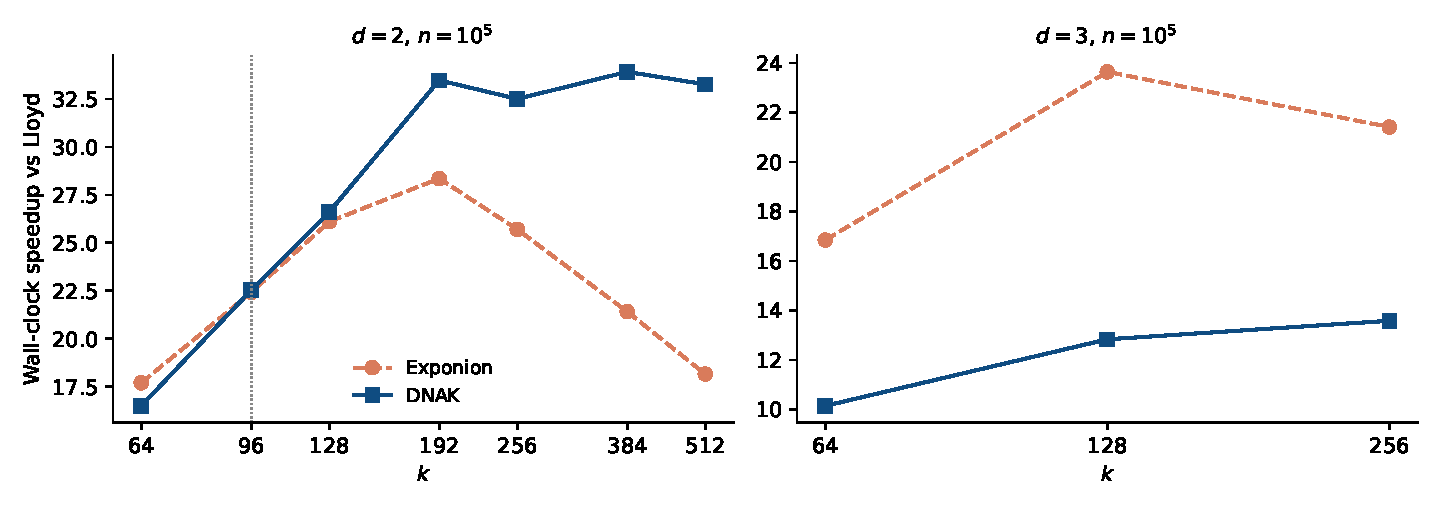
\includegraphics[width=\linewidth]{crossover.pdf}
\caption{Wall-clock speedup versus Lloyd's algorithm as $k$ grows
($n=10^5$). In the plane (left), DNAK overtakes Exponion at
$k^\ast\approx 96$ and the margin widens to $1.8\times$ at $k{=}512$;
at $d{=}3$ (right) Exponion remains ahead at the tested $k$, with the
ratio narrowing as $k$ grows.}
\label{fig:cross}
\end{figure}

% =====================================================================
\section{Limitations}
\label{sec:limits}

Three limitations bound our claims. (i)~\emph{Graph construction
cost.} DNAK rebuilds the exact Delaunay graph of the centroids every
iteration; this is cheap in the plane but its
$O(k^{\lceil d/2\rceil})$ growth already erodes the wall-clock
advantage at $d{=}4$ and confines the present method to low dimension
($d\le 4$), a regime that nonetheless covers geospatial analytics,
colour quantisation and low-dimensional embeddings. Incremental
maintenance of the graph under small centroid drift, or replacing it
with a Gabriel or centroid-$k$NN graph whose walk result is certified
by the maintained bounds (with an exact full-scan fallback), are the
natural remedies and are left to future work. (ii)~\emph{Baseline
scope.} Ball $k$-means \cite{ballkmeans}, the closest
neighbour-restricted method, is not yet included as an experimental
baseline; its comparison, along with the UCI 3D Road Network dataset,
is planned for the camera-ready version. (iii)~\emph{Protocol.}
Exactness on tie-degenerate data holds relative to the declared
tie-breaking rule, and our Yinyang and Exponion numbers reflect our
own implementations of the published constructions rather than the
authors' optimised code, which is why distance computations serve as
the metric of record.

% =====================================================================
\section{Conclusion}
\label{sec:conc}

DNAK shows that the computational geometry of the evolving centroid
set --- Delaunay adjacency, order-2 Voronoi structure and greedy walks
--- yields an exact $k$-means accelerator with $O(n)$ memory, provably
minimal structural candidate sets and exact second-nearest bounds. In
a verified six-method comparison it consistently outperforms
Hamerly's, Elkan's and Yinyang's algorithms in wall-clock terms, and a
$k$-sweep establishes that in the plane it overtakes Exponion at
$k^\ast\approx 96$ and widens its lead to $1.8\times$ by $k{=}512$,
making DNAK, to our knowledge, the fastest exact method for large-$k$
planar clustering; at $d{=}3$ the remaining gap is localised to graph
reconstruction, whose certificate-gated lazy variant we analysed and
reported as a negative result. Beyond the algorithm, these results
substantiate the broader thesis claim that Euclidean and computational
geometry supplies exact, quantifiable optimisation machinery for
centroid-based clustering.

\section*{Declaration of competing interest}
The authors declare no competing interests.

\section*{Data availability}
Reference implementation and experiment scripts to be released at
[TODO: repository URL].

\begin{thebibliography}{99}
\bibitem{lloyd} S.~Lloyd, Least squares quantization in PCM, IEEE
Trans.\ Inf.\ Theory 28(2) (1982) 129--137.
\bibitem{elkan} C.~Elkan, Using the triangle inequality to accelerate
$k$-means, ICML (2003).
\bibitem{hamerly} G.~Hamerly, Making $k$-means even faster, SDM (2010).
\bibitem{drake} J.~Drake, G.~Hamerly, Accelerated $k$-means with
adaptive distance bounds, 5th NIPS Workshop on Optimization for
Machine Learning (2012).
\bibitem{yinyang} Y.~Ding et al., Yinyang $k$-means: a drop-in
replacement of the classic $k$-means with consistent speedup, ICML
(2015).
\bibitem{hamerlydrake} G.~Hamerly, J.~Drake, Accelerating Lloyd's
algorithm for $k$-means clustering, in: Partitional Clustering
Algorithms, Springer (2015) 41--78.
\bibitem{newling} J.~Newling, F.~Fleuret, Fast $k$-means with accurate
bounds, ICML (2016).
\bibitem{bottesch} T.~Bottesch, T.~B\"uhler, M.~K\"achele, Speeding up
$k$-means by approximating Euclidean distances via block vectors,
ICML (2016).
\bibitem{rysavy} P.~Ry\v{s}av\'{y}, G.~Hamerly, Geometric methods to
accelerate $k$-means algorithms, SDM (2016) 324--332.
\bibitem{borgelt} C.~Borgelt, Even faster exact $k$-means clustering,
Advances in Intelligent Data Analysis XVIII (IDA), LNCS 12080,
Springer (2020) 93--105.
\bibitem{wang21} S.~Wang, Y.~Sun, Z.~Bao, On the efficiency of
$k$-means clustering: evaluation, optimization, and algorithm
selection, Proc.\ VLDB Endow.\ 14(2) (2021) 163--175.
\bibitem{schubert} E.~Schubert, A.~Lang, G.~Feher, Accelerating
spherical $k$-means, Similarity Search and Applications (SISAP),
Springer (2021).
\bibitem{raff} E.~Raff, Exact acceleration of $k$-means++ and
$k$-means$\|$, IJCAI (2021) 2928--2935.
\bibitem{ballkmeans} S.~Xia, D.~Peng, D.~Meng, C.~Zhang, G.~Wang,
E.~Giem, W.~Wei, Z.~Chen, Ball $k$-means: fast adaptive clustering
with no bounds, IEEE Trans.\ Pattern Anal.\ Mach.\ Intell.\ 44(1)
(2022) 87--99.
\bibitem{corominas} G.~Rodr\'iguez Corominas, M.~J.~Blesa, C.~Blum,
Accelerating the $k$-means++ algorithm by using geometric
information, arXiv:2408.13189 (2024).
\bibitem{pelleg} D.~Pelleg, A.~Moore, Accelerating exact $k$-means
algorithms with geometric reasoning, KDD (1999) 277--281.
\bibitem{kanungo} T.~Kanungo et al., An efficient $k$-means clustering
algorithm: analysis and implementation, IEEE TPAMI 24(7) (2002).
\bibitem{aurenhammer} F.~Aurenhammer, Voronoi diagrams --- a survey of
a fundamental geometric data structure, ACM Comput.\ Surv.\ 23(3)
(1991).
\bibitem{arthur} D.~Arthur, S.~Vassilvitskii, $k$-means++: the
advantages of careful seeding, SODA (2007).
\end{thebibliography}
\end{document}
